\documentclass{article}

\usepackage{amsmath}
\usepackage{amssymb}
\usepackage{parskip}
\usepackage{hyperref}
\usepackage{fullpage}
\usepackage{tikz}
\usepackage{float}

\usepackage{notepiece}

\hypersetup{
    colorlinks=true,
    linkcolor=black,
    urlcolor=blue,
    pdftitle={Test},
    pdfpagemode=FullScreen,
}

\newcommand{\integral}[4]{\int\limits_{#1}^{#2} #3\,d#4}
    
\begin{document}

\begin{minipage}{0.5\textwidth}
    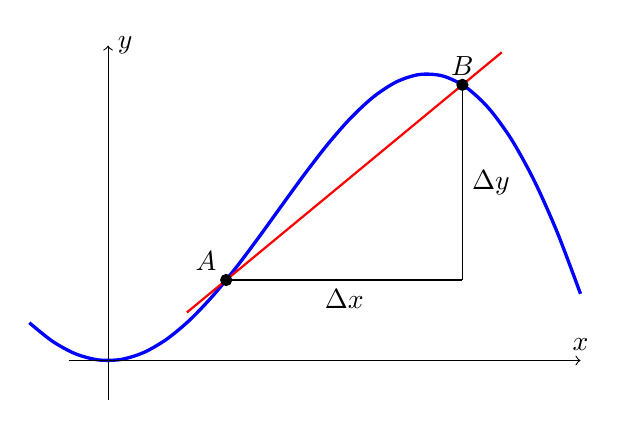
\begin{tikzpicture}[
        scale=2,
        declare function={
            func(\x) = \x*sin(\x r);
            Width=3;
            Height=2;
            Ax=0.75;
            Bx=2.25;
            SlopeMargin=0.25;
            M=(func(Bx) - func(Ax)) / (Bx - Ax);
            Q=func(Ax) - M * Ax;
            slopeFunc(\x)=\x * M + Q;
        }
    ]
        \draw[domain=-0.5:3, smooth, variable=\x, blue, very thick] plot ({\x}, {func(\x)});
        
        \draw[->] (0, -0.25) -- (0, Height) node[right] {\(y\)};
        \draw[->] (-0.25, 0) -- (Width, 0) node[above] {\(x\)};

        \draw[-] (Ax, {func(Ax)}) -- node[below] {\(\Delta x\)} (Bx, {func(Ax)});
        \draw[-] (Bx, {func(Ax)}) -- node[right] {\(\Delta y\)} (Bx, {func(Bx)});
        
        \filldraw [red, thick] ({Ax - SlopeMargin}, {slopeFunc(Ax - SlopeMargin)}) -- ({Bx + SlopeMargin}, {slopeFunc(Bx + SlopeMargin)});
        
        \filldraw (Ax,{func(Ax)}) circle (1pt) node[above left] {\(A\)};
        \filldraw (Bx,{func(Bx)}) circle (1pt) node[above] {\(B\)};
    \end{tikzpicture}
\end{minipage}
\begin{minipage}{0.5\textwidth}
    The mean slope of a function \(f\) between a point \(A\) and \(B\) is given by
    \[
        \frac{\Delta y}{\Delta x} = \frac{f(B)-f(A)}{B-A}
    \]
    As we make \(A\) and \(B\) closer to eachother, \(\Delta x\) decreases.
    As \(\Delta x\) decreases the mean slope is more representative of the rate of change
    of \(f\) in the interval \([A;B]\). \\
\end{minipage}

\begin{minipage}{0.5\textwidth}
    When \(\Delta x\) is infinitely small, we have the precise slope of a given point
    on the function. This slope is represented by the tangent line, which is parallel to the given point.
    \[
        \lim_{\Delta x \to 0} \frac{\Delta x}{\Delta x}
    \]
\end{minipage}
\begin{minipage}{0.5\textwidth}
    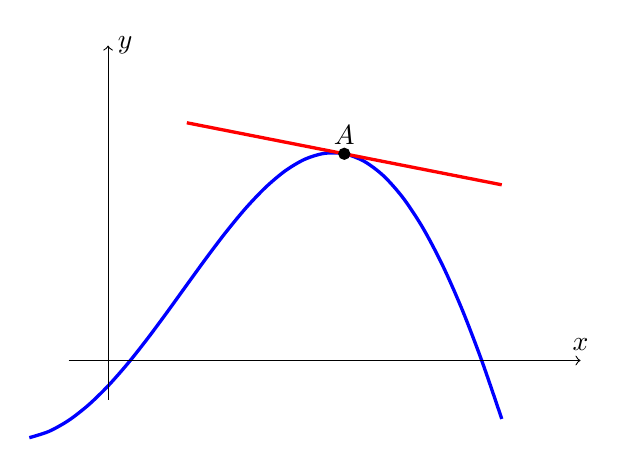
\begin{tikzpicture}[
        scale=2,
        declare function={
            func(\x) = (\x+0.6)*sin((\x+0.6) r)-0.5;
            Width=3;
            Height=2;
            Ax=1.5;
            slope = -0.19697;
        }
    ]
        \draw[domain=-0.5:2.5, smooth, variable=\x, blue, very thick] plot ({\x}, {func(\x)});
        
        \draw[->] (0, -0.25) -- (0, Height) node[right] {\(y\)};
        \draw[->] (-0.25, 0) -- (Width, 0) node[above] {\(x\)};

        \draw[domain=0.5:2.5, smooth, variable=\x, red, very thick] plot ({\x}, {slope * \x + func(Ax) - slope * Ax});
        
        \filldraw (Ax,{func(Ax)}) circle (1pt) node[above] {\(A\)};
    \end{tikzpicture}
\end{minipage}

\end{document}